% !TEX root = ../tex/4-2.tex
% 第4章：本文は青、補足は緑
\newcommand{\asmain}{%
    \setbeamercolor{frametitle}{fg=white,bg=main}%
    \setbeamercolor{structure}{fg=main}%
    \setbeamercolor{itemize item}{fg=main}%
    \setbeamercolor{itemize subitem}{fg=main}%
    \setbeamercolor{enumerate item}{fg=main}%
}
\newcommand{\assuppl}{%
    \setbeamercolor{frametitle}{fg=white,bg=examplecol}%
    \setbeamercolor{structure}{fg=examplecol}%
    \setbeamercolor{itemize item}{fg=examplecol}%
    \setbeamercolor{itemize subitem}{fg=examplecol}%
    \setbeamercolor{enumerate item}{fg=examplecol}%
}
% フレームタイトルの「補足」だけを□で囲む
\newcommand{\supplmark}{%
    \setlength{\fboxsep}{1.5pt}%
    \setlength{\fboxrule}{0.7pt}%
    \fbox{\textbf{補足}}%
}
\asmain


%=============================================
\begin{frame}{4.1から4.2へ}
    \begin{block}{ここまで（4.1）}
        前向きSDEが周辺$\{p_t\}$を定義し、\\
        逆時間SDE／PF-ODEはスコア$\nabla_{\bm{x}}\log p_t$で生成する。\\
        周辺は揃うが、軌跡の法則は違ってよい。
    \end{block}
    \begin{block}{ここから（4.2＝論文4.3）}
        時間条件付きネット$s_\phi(\bm{x},t)$をDSMで学習する。\\
        学習スコアを逆SDE／PF-ODEに入れてサンプルし、\\
        PF-ODEでは尤度評価もできる。
    \end{block}
\end{frame}
%=============================================
\asmain
\begin{frame}{4.2 の位置づけ}
    \begin{block}{この節の役割}
        原理（SDE／ODE）を、学習とサンプリングの手続きに落とす
    \end{block}
    \begin{enumerate}
        \item \textbf{学習}\\
        時間依存DSM（式4.3.1）と最適解（命題4.3.1）
        \item \textbf{サンプリング}\\
        経験逆時間SDE（4.3.3）（4.3.4）と経験PF-ODE（4.3.5）（4.3.6）
        \item \textbf{尤度}\\
        前向きPF-ODE＋変数変換（式4.3.7）
    \end{enumerate}
    \vfill
    \footnotesize
    フォルダ字幕は「4.2 Training and Sampling」。内容は論文§4.3。
\end{frame}
%=============================================
\section{学習（DSM）}
\asmain
\begin{frame}{区切り：学習（DSM）}
    \tableofcontents[currentsection]
\end{frame}
%=============================================
\asmain
\begin{frame}{時間条件付きスコアネット}
    第3章と同じ思想で、オラクル$\nabla_{\bm{x}}\log p_t(\bm{x})$を
    \[
        s_\phi=s_\phi(\bm{x},t)
        \qquad(t\in[0,T])
    \]
    で近似する。素朴なスコアマッチングは
    \[
        \resizebox{0.98\textwidth}{!}{$
        \mathcal{L}_{\mathrm{SM}}(\phi;\omega)
        :=
        \dfrac12
        \mathbb{E}_{t\sim p_{\mathrm{time}}}
        \mathbb{E}_{\bm{x}_t\sim p_t}
        \bigl[
        \omega(t)\,
        \|s_\phi(\bm{x}_t,t)-\nabla_{\bm{x}}\log p_t(\bm{x}_t)\|_{2}^{2}
        \bigr]
        $}
    \]
    だが、教師$\nabla\log p_t$は一般に未知である。
\end{frame}
%=============================================
\asmain
\begin{frame}{図4.6：DSMのトリック}
    \centering
    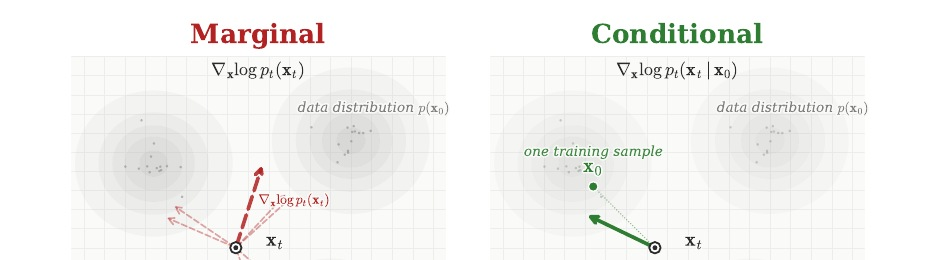
\includegraphics[width=\textwidth,height=0.62\textheight,keepaspectratio]{fig-4-6.jpg}
    \vfill
    \footnotesize
    左：周辺スコアは全データの寄与の和で扱いづらい。\\
    右：訓練時は$\bm{x}_0$が分かるので、条件付きスコアが閉じた教師になる。
\end{frame}
%=============================================
\assuppl
\begin{frame}{\supplmark：図4.6の読み方}
    \begin{columns}[T,onlytextwidth]
        \begin{column}{0.48\textwidth}
            \begin{exampleblock}{左（周辺）}
                固定$\bm{x}_t$への寄与を、\\
                あり得るきれいな$\bm{x}_0$全体で足す必要がある。
            \end{exampleblock}
        \end{column}
        \begin{column}{0.48\textwidth}
            \begin{exampleblock}{右（条件付き）}
                そのサンプルを作った$\bm{x}_0$だけを使う。\\
                ガウス摂動なら教師は明示できる。
            \end{exampleblock}
        \end{column}
    \end{columns}
    \vspace{0.35em}
    \begin{exampleblock}{平均の意味}
        条件付きスコアを多くの$(\bm{x}_0,\bm{x}_t)$で回帰すると、\\
        平均的には周辺スコアに一致する。
    \end{exampleblock}
\end{frame}
%=============================================
\asmain
\begin{frame}{連続時間のDSM損失}
    \[
        \resizebox{0.98\textwidth}{!}{$
        \begin{aligned}
        &\mathcal{L}_{\mathrm{DSM}}(\phi;\omega)
        :=\\
        &\quad
        \dfrac12
        \mathbb{E}_{t}
        \mathbb{E}_{\bm{x}_0}
        \mathbb{E}_{p_t(\bm{x}_t|\bm{x}_0)}
        \Bigl[
        \omega(t)\,
        \bigl\|
        s_\phi(\bm{x}_t,t)
        -
        \nabla_{\bm{x}_t}\log p_t(\bm{x}_t|\bm{x}_0)
        \bigr\|_{2}^{2}
        \Bigr]
        \end{aligned}
        $}
        \tag{4.3.1}
    \]
    \begin{block}{読み方}
        離散NCSNの和（3.4.1）の連続版。\\
        和$\sum_i$が時間期待$\mathbb{E}_t$に置き換わる。
    \end{block}
\end{frame}
%=============================================
\asmain
\begin{frame}{命題4.3.1：DSMの最小化子}
    最小化子$s^{\star}$は、ほとんどすべての$\bm{x}_t\sim p_t$と$t$について
    \[
        \resizebox{0.98\textwidth}{!}{$
        s^{\star}(\bm{x}_t,t)
        =
        \mathbb{E}_{\bm{x}_0\sim p(\bm{x}_0|\bm{x}_t)}
        \bigl[
        \nabla_{\bm{x}_t}\log p_t(\bm{x}_t|\bm{x}_0)
        \bigr]
        =
        \nabla_{\bm{x}_t}\log p_t(\bm{x}_t)
        $}
        \tag{4.3.2}
    \]
    \begin{block}{意味}
        条件付きスコアへの回帰でも、欲しい周辺スコアが一意に得られる。\\
        （定理3.3.1の連続時間版）
    \end{block}
\end{frame}
%=============================================
\asmain
\begin{frame}{学習のまとめ}
    \begin{itemize}
        \item ネットは$s_\phi(\bm{x},t)$：時刻を条件にする
        \item 実用はDSM（4.3.1）。教師は$\nabla\log p_t(\bm{x}_t|\bm{x}_0)$
        \item 最適解は周辺スコアそのもの（4.3.2）
    \end{itemize}
    \begin{block}{次}
        学習スコアを逆時間SDE／PF-ODEに代入してサンプルする。
    \end{block}
\end{frame}
%=============================================
\section{サンプリング}
\asmain
\begin{frame}{区切り：サンプリング}
    \tableofcontents[currentsection]
\end{frame}
%=============================================
\asmain
\begin{frame}{経験逆時間SDE}
    $s_{\phi^\star}(\bm{x},t)\approx\nabla_{\bm{x}}\log p_t(\bm{x})$を式（4.1.6）へ代入：
    \[
        \resizebox{0.98\textwidth}{!}{$
        d\bm{x}^{\mathrm{SDE}}(t)
        =
        \bigl[
        \bm{f}(\bm{x}^{\mathrm{SDE}}(t),t)
        -
        g^{2}(t)\,s_{\phi^\star}(\bm{x}^{\mathrm{SDE}}(t),t)
        \bigr]dt
        +
        g(t)\,d\bar{\bm{w}}(t)
        $}
        \tag{4.3.3}
    \]
    $\bm{x}_T\sim p_{\mathrm{prior}}$から$t=T\to 0$と数値積分する。
\end{frame}
%=============================================
\asmain
\begin{frame}{Euler--Maruyama更新}
    ステップ幅$\Delta t>0$、$\bm{\epsilon}\sim\mathcal{N}(\bm{0},\bm{I})$として
    \[
        \resizebox{0.98\textwidth}{!}{$
        \bm{x}_{t-\Delta t}
        \leftarrow
        \bm{x}_t
        -
        \bigl[
        \bm{f}(\bm{x}_t,t)
        -
        g^{2}(t)\,s_{\phi^\star}(\bm{x}_t,t)
        \bigr]\Delta t
        +
        g(t)\sqrt{\Delta t}\,\bm{\epsilon}
        $}
        \tag{4.3.4}
    \]
    \begin{block}{結果}
        最終状態の分布$p_{\phi^\star}^{\mathrm{SDE}}(\cdot;0)\approx p_{\mathrm{data}}$。\\
        VP構成では、DDPMサンプリングの連続極限と一致する（4.4）。
    \end{block}
\end{frame}
%=============================================
\asmain
\begin{frame}{図4.7：逆SDEとPF-ODEの軌跡}
    \centering
    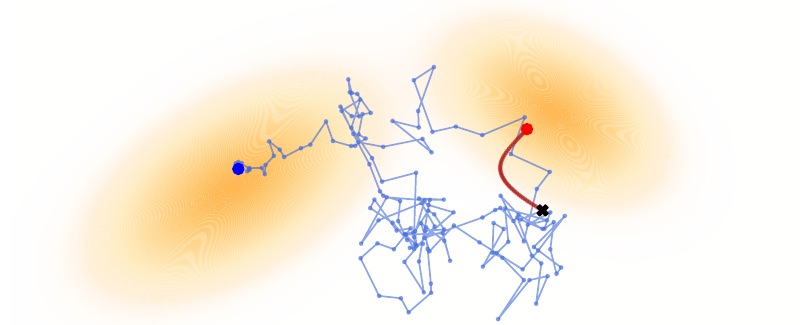
\includegraphics[width=\textwidth,height=0.62\textheight,keepaspectratio]{fig-4-7.jpg}
    \vfill
    \footnotesize
    青：逆時間SDE（確率的）。赤：PF-ODE（確定的）。\\
    どちらも$t\to 0$で$p_{\mathrm{data}}$の支持へ向かう。
\end{frame}
%=============================================
\assuppl
\begin{frame}{\supplmark：図4.7の設定}
    \begin{exampleblock}{前向き}
        $d\bm{x}=\sqrt{2t}\,d\bm{w}$（$\bm{f}\equiv\bm{0}$）。\\
        2峰混合$p_0$が$p_T\approx\mathcal{N}(\bm{0},T^{2}\bm{I})$へ広がる。
    \end{exampleblock}
    \begin{exampleblock}{生成}
        暗い$\times$が$\bm{x}_T\sim p_{\mathrm{prior}}$。\\
        青は式（4.3.4）、赤は式（4.3.6）の数値解。
    \end{exampleblock}
    \begin{exampleblock}{読み方}
        周辺は同じでも、1本の道のりは確率的と確定的で見た目が違う。
    \end{exampleblock}
\end{frame}
%=============================================
\asmain
\begin{frame}{経験PF-ODEによるサンプリング}
    式（4.1.7）のスコアを$s_{\phi^\star}$に置換：
    \[
        \frac{d\bm{x}^{\mathrm{ODE}}(t)}{dt}
        =
        \bm{f}(\bm{x}^{\mathrm{ODE}}(t),t)
        -
        \tfrac12 g^{2}(t)\,
        s_{\phi^\star}(\bm{x}^{\mathrm{ODE}}(t),t)
        \tag{4.3.5}
    \]
    Euler法では
    \[
        \bm{x}_{t-\Delta t}
        \leftarrow
        \bm{x}_t
        -
        \Bigl[
        \bm{f}(\bm{x}_t,t)
        -
        \tfrac12 g^{2}(t)\,s_{\phi^\star}(\bm{x}_t,t)
        \Bigr]\Delta t
        \tag{4.3.6}
    \]
\end{frame}
%=============================================
\asmain
\begin{frame}{Insight：生成＝ODE／SDEを解くこと}
    \begin{block}{Insight 4.3.1}
        拡散モデルからのサンプリングは、\\
        本質的に確率流ODEまたは逆時間SDEを解くことと等価である。
    \end{block}
    \begin{itemize}
        \item だから反復が多く、生成が遅い（第3章の問いへの答え）
        \item 一方で、ODE加速の文献をそのまま借りやすい（第9章）
        \item 典型的には数千回の関数評価が使われる例が多い
    \end{itemize}
\end{frame}
%=============================================
\asmain
\begin{frame}{サンプリングのまとめ}
    \begin{itemize}
        \item 逆SDE：式（4.3.3）をEuler--Maruyama（4.3.4）で$T\to 0$
        \item PF-ODE：式（4.3.5）をEuler（4.3.6）などで$T\to 0$
        \item 生成コストの本体は、微分方程式の反復求解である
    \end{itemize}
    \begin{block}{次}
        同じPF-ODEで、符号化と尤度評価もできる。
    \end{block}
\end{frame}
%=============================================
\section{反転と尤度}
\asmain
\begin{frame}{区切り：反転と尤度}
    \tableofcontents[currentsection]
\end{frame}
%=============================================
\asmain
\begin{frame}{PF-ODEの反転（符号化）}
    SDEと違い、同じ式（4.3.5）を$0\to T$にも解ける。
    \begin{block}{前向きに解く}
        データ$\bm{x}_0$を、各$t$の潜在表現へ運ぶ（エンコーダ）。\\
        画像翻訳・編集など、制御可能な生成の土台になる。
    \end{block}
    \begin{block}{逆向きに解く}
        事前からデータへ戻す（通常の生成）。
    \end{block}
\end{frame}
%=============================================
\asmain
\begin{frame}{尤度：変数変換に沿った密度の変化}
    学習済み速度場
    \[
        \bm{v}_{\phi^\star}(\bm{x},t)
        :=
        \bm{f}(\bm{x},t)
        -
        \tfrac12 g^{2}(t)\,s_{\phi^\star}(\bm{x},t)
    \]
    に沿う軌跡では
    \[
        \frac{d}{dt}
        \log p_{\phi^\star}^{\mathrm{ODE}}(\bm{x}(t);t)
        =
        -\nabla_{\bm{x}}\cdot\bm{v}_{\phi^\star}(\bm{x}(t),t)
    \]
    状態と対数密度の増分を同時に積分できる。
\end{frame}
%=============================================
\asmain
\begin{frame}{式（4.3.7）：同時積分}
    \[
        \frac{d}{dt}
        \begin{bmatrix}
        \bm{x}(t)\\
        \delta(t)
        \end{bmatrix}
        =
        \begin{bmatrix}
        \bm{v}_{\phi^\star}(\bm{x}(t),t)\\
        -\nabla_{\bm{x}}\cdot\bm{v}_{\phi^\star}(\bm{x}(t),t)
        \end{bmatrix},
        \quad
        \begin{bmatrix}
        \bm{x}(0)\\
        \delta(0)
        \end{bmatrix}
        =
        \begin{bmatrix}
        \bm{x}_0\\
        0
        \end{bmatrix}
        \tag{4.3.7}
    \]
    $t=T$で$p_{\mathrm{prior}}(\bm{x}(T))$が既知なので
    \[
        \log p_{\phi^\star}^{\mathrm{ODE}}(\bm{x}_0;0)
        =
        \log p_{\mathrm{prior}}(\bm{x}(T))-\delta(T)
    \]
\end{frame}
%=============================================
\assuppl
\begin{frame}{\supplmark：積分形での尤度}
    同等に
    \[
        \log p_{\phi^\star}^{\mathrm{ODE}}(\bm{x}_0;0)
        =
        \log p_{\mathrm{prior}}(\bm{x}(T))
        +
        \int_0^T
        \nabla_{\bm{x}}\cdot\bm{v}_{\phi^\star}(\bm{x}(t),t)\,
        dt
    \]
    \begin{exampleblock}{要点}
        生成・反転に使う同じPF-ODEが、\\
        連続の変数変換公式として尤度も与える。
    \end{exampleblock}
\end{frame}
%=============================================
\asmain
\begin{frame}{反転・尤度のまとめ}
    \begin{itemize}
        \item PF-ODEは$0\leftrightarrow T$の双方向流である
        \item 前向き流は潜在符号化、逆向き流は生成
        \item 発散の積分で$\log p(\bm{x}_0)$を評価できる（4.3.7）
    \end{itemize}
\end{frame}
%=============================================
\asmain
\begin{frame}{4.2 全体のまとめ}
    \begin{enumerate}
        \item \textbf{学習}
        連続DSM（4.3.1）で$s_\phi(\bm{x},t)$を学ぶ。最適は周辺スコア。
        \item \textbf{生成}
        逆SDE（4.3.3–4.3.4）またはPF-ODE（4.3.5–4.3.6）を解く。
        \item \textbf{尤度}
        同じPF-ODEの発散積分（4.3.7）で$\log p$が取れる。
        \item \textbf{含意}
        生成の遅さは、DEソルバの反復コストそのものである。
    \end{enumerate}
\end{frame}
%=============================================
\asmain
\begin{frame}{4.2 全体のまとめ：一本の流れ}
    \begin{block}{今日の道筋}
        時間依存スコアをDSMで学ぶ
        $\;\to\;$
        逆SDE／PF-ODEでサンプル
        $\;\to\;$
        PF-ODEで符号化・尤度
    \end{block}
    \begin{block}{核心}
        原理は「スコアを入れた微分方程式」。\\
        実装は「条件付き教師で回帰し、数値積分する」こと。
    \end{block}
    \begin{block}{次へ}
        4.3ではVE／VPなど、前向きSDEの具体的な選び方（インスタンス）を見る。
    \end{block}
\end{frame}
